\def \DocType{		%Problem Statement
				%Requirements Document
				%Technology Review
				Design Document
				%Progress Report
				}

\begin{titlepage}
    \pagenumbering{gobble}
    \begin{singlespace}
    	
\includegraphics[height=4cm]{coe_v_spot1}
        \hfill 
        % 4. If you have a logo, use this includegraphics command to put it on the coversheet.
        %\includegraphics[height=4cm]{CompanyLogo}   
        \par\vspace{.2in}
        \centering
        \scshape{
            \huge CS Capstone \DocType \par
            {\large\today}\par
            \vspace{.5in}
            \textbf{\Huge\CapstoneProjectName}\par
            \vfill
            {\large Prepared for}\par
            \Huge \CapstoneSponsorCompany\par
            \vspace{5pt}
            {\Large
                \NameSigPair{\CapstoneSponsorPersonTwo}\par
            }
            {\large Prepared by }\par
            Group\CapstoneTeamNumber\par
            % 5. comment out the line below this one if you do not wish to name your team
            \CapstoneTeamName\par 
            \vspace{5pt}
            {\Large
                \NameSigPair{\GroupMemberOne}\par
                \NameSigPair{\GroupMemberTwo}\par
                \NameSigPair{\GroupMemberThree}\par
            }
            \vspace{20pt}
        }
        \begin{abstract}
        % 6. Fill in your abstract    
This project involves solving the problem of some universities lacking resources to visually show physical and mechanical interactions for Mechanical Engineering concepts.
This project is built on the research that shows that students can achieve a better understanding of difficult concepts by learning through interactive simulated environments.
By implementing 2D simulations based on these concepts, students will be able to visually interpret the concepts in the course.
The goal of this document is to document the design for these 2D simulations, explaining the implementations of the features which shall be expected for this project.
        \end{abstract}     
    \end{singlespace}
\end{titlepage}
\newpage
%\pagenumbering{arabic}
%\tableofcontents
% 7. uncomment this (if applicable). Consider adding a page break.
%\listoffigures
%\listoftables
\clearpage

% 8. now you write!
%Create NEW DRAFTs of your requirements and design documents that include the following contents.

%(1) a table of changes made to the original requirements and/or design, placed right AFTER the table of contents in each of the two papers (three columns in the table should be labeled [section] [original] [new]; the rows should include bullet points with changes)

%(2) changes to detailed content in the document, itself

%(3) a new file name that includes your team name, type of document, and draft number

\section{Revision Table}
\begin{table}[H]
  \centering
  \caption{Revisions}
  \label{my-label}
  \begin{tabular}{|p{0.1\linewidth}|p{0.4\linewidth}|p{0.4\linewidth}|}
    \hline
    \textbf{Section} & \textbf{Original} & \textbf{New} \\
    \hline
    %a table of changes made to the original requirements and/or design, placed right AFTER the table of contents in each of the two papers (three columns in the table should be labeled [section] [original] [new]; the rows should include bullet points with changes)

    % ************ Revision 1******************%
    4.3 & 
    %%
    Described the game engine, Defold & 
    %%
    Describes the physics engine, Matter.js \\
    \hline
    % ************ Revision 2 ****************%
    4.4.3 &
    %%
    \begin{itemize}
        \item Exploratory mode description using Defold's input system and collision object feature
        \item Use Bootstrap to design the webpage
    \end{itemize}
     &
    %%
    \begin{itemize}
        \item Used matter.js to control all the inputs into the pendulum system
        \item Used the library noUiSlider to receive input 
        \item Used HTML and CSS to design the webpage of each simulation
    \end{itemize}\\
    \hline
    % ************ Revision 3 ****************%
    4.6 &
    %%
    Art Software &
    %%
    This section is removed since we are using the built in 
    entities provided by the Matter.js library.\\
    \hline


    

  \end{tabular}
\end{table}

\section{Overview}
This document contains an in depth description of the designs to be used in the 2D Simulations for Inquiry-Based Learning project. This document will go over the UI design layouts needed for the simulation web page, the implementation of web page hosting, and the implementation of the animation. The components within each of these sections are also explained. 

\subsection{Scope}
Our product will consist of six variations of a two dimensional simulation based on mechanical engineering concepts in order to support inquiry based learning for mechanical engineering students. The simulations will be hosted on the Concept Warehouse website, which is a website that provides interactive learning opportunities for classrooms. While the simulation is running, real time mathematical feedback will be provided in the form of graphs or simply values in the simulation. There will be start, stop, and reset button within each simulation so that the student can explore the simulations as many times or at as many points as they need to. The students will also be able to modify specific parameters within the sixth variation of the simulation, such as mass, friction, and angles.

\subsection{Purpose}
The purpose of this document is to present the design specifications for the Interactive 2D Simulations to support Inquiry-Based Learning in Mechanical Engineering project. This document will expand on the technologies used to implement the project, which will include:

\begin{itemize}
  \item The process of serving the simulations to the student
  \item The Physics Engine used to procure the simulations
  \item User Interface designs for the web page
  \item Data Visualization
  \item Software for creating the simulation assets
\end{itemize} 

\subsection{Intended Audience}
The intended audience for this document is primarily for developers that will be working on the project and need to be on boarded. In addition to this, the document is used as verification to the client's of the project, Milo Koretsky and Tom Ekstedt, to make sure that the design falls inline with the expectations they have provided.


\section{Glossary}
\begin{itemize}
  \item Concept Warehouse - A platform for engineering students to answer questions inside or outside of class.
  \item User Interface (UI) - The aspect of a program that the user interacts with directly through keyboard and mouse.
  \item Simulation - A digital and visual representation of a physics model.
  \item Object - A particular instance of a class, where the object can be a combination of variables, functions, and data structures.
  \item JavaScript - A core scripting language used in the web. It is used to create interactive elements within a web page.
  \item Chart.js - A lightweight JavaScript library for creating interactive graphs and that is free to use for the web.
  \item Open-source - Software code that has been made available for public use and manipulation.
  \item Matter.js - A free, 2D physics engine, based on Box2D; a C++ physics engine.
  \item Coefficient of Restitution - ratio of the final to initial relative velocity between two objects after collision. Values range from 0 to 1
  \item Mockup - A prototype providing the design and functionality of a system 
\end{itemize} 

\subsection{Design Timeline}
\begin{itemize}
    \item Jan 7 - Jan 20: UI creation
    \item Jan 20 - Feb 20: Simulation creation
    \item Feb 20 - Mar 22: Graph Add-on and Bug Fixes
    \item Mar 22 - April 10: Clean Up and Stretch Goals
    \item April 10 - Expo: Expo Preparation
\end{itemize}
% general timeline 

\section{Design Viewpoints}
%Example: http://user.ceng.metu.edu.tr/~e1819002/SDD.pdf

\subsection{Introduction}
The different components of the web page is the hosting information, physics engine, user interface, graphs, and art software. The following section explains each of the components and the implementation design. 
%********************************************
% Hosting information
%********************************************
\subsection{Hosting}
The project will consist of several files that will be delivered to the client. The client will then upload these files to their own server to be distributed to students. The end product will simply be a simulation that can be displayed to students.
The simulation consists of 5 pendulum variation cases and an exploratory mode. The flow of the system is that the instructor dictates when students are able to view the simulation through Concept Warehouse. Then the server updates the content of the web page with a new case. The cases are shown in sequential order from 1 to 5. Exploratory mode, where users can modify parameters, is also unlocked by the instructor. 

\begin{figure}[H]
  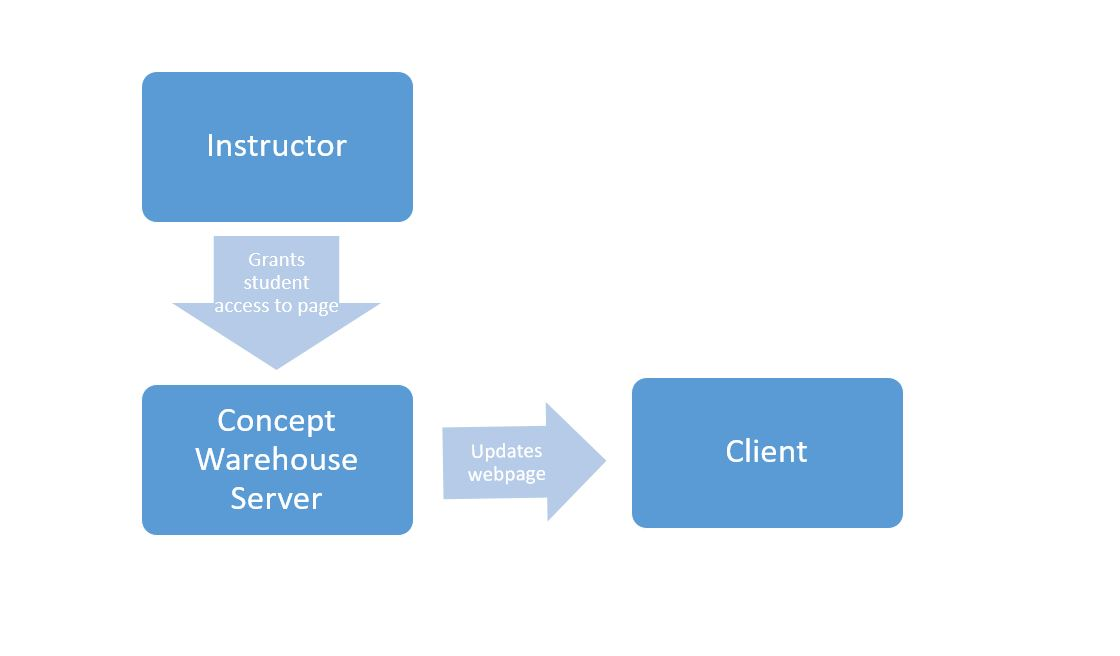
\includegraphics[width=6.5 in]{hosting_diagram.eps}
  \caption{Hosting Diagram}
  \label{fig:host}
\end{figure}

%********************************************
% Physics Engine
%********************************************
\subsection{Viewpoint: Physics Engine}
%can add other subsections

\subsubsection{Design Concerns}
Creating the physics needed to accurately portray pendulums acting upon each other would take more time and knowledge than what we currently have. Using an open source physics engine will allow us to create the simulations very quickly.

\subsubsection{Design Elements}
Physics engines are pre-made frameworks that allow for fast creation of physics objects, which respond to each other in a realistic way. Primarily, these objects are referred to as "bodies," and they hold specific properties, such as position, velocity, mass, and friction constants. The physics engine we chose is Matter.js, which is based off of Box2D, a well known, C++ physics engine. Matter.js is open source, which means we do not need to worry about a paid license to use the engine.

\subsubsection{Function Attribute}
The physics engine, Matter.js, will allow the team to quickly create multiple simulations of similar types. The ability to visually create physics objects with a few lines of code will greatly increase our productivity.
\newline

%%
% insert more info about matter.js wth example code: 
%%

%********************************************
%  User interface
%********************************************
\subsection{Viewpoint: User Interface}
The User Interface is the gateway to connecting with the end user. It allows for interactivity with the simulation.
%can add other subsections

\subsubsection{Design Concerns}
A disorganized UI or a UI that is hard to understand can impede the student's learning. Even if the animation runs well in itself, if the web page it is placed in is hard to manipulate, it can take away from the animation. 

\subsubsection{Function Attribute: Normal Mode}
The user interface mockup of Case 1 is shown in Figure \ref{fig:case1_start} and Figure \ref{fig:case1_end}. Figure \ref{fig:case1_start} will be the initial screen shown. This will be the normal mode of case 1. Normal mode is applicable to all 5 of the variations of the impact pendulum scenario. 
The normal mode components with their description are as such:
\begin{itemize}
    \item Start/Pause Button - Starts the simulation or pauses it 
    \item Reset Button - Resets the simulation
    \item Graph of angle vs. time 
    \item Live measurement updates  - Updates the angle and height of each weight, velocity, and the time every 0.1 seconds of the simulation
    \item Starting measurements  - Length (m), weight (g), angle (degrees), height of weight off the ground (m), and coefficient of restitution 
\end{itemize}

The graph component design is explained in section 3.5. \newline


\begin{figure}[H]
  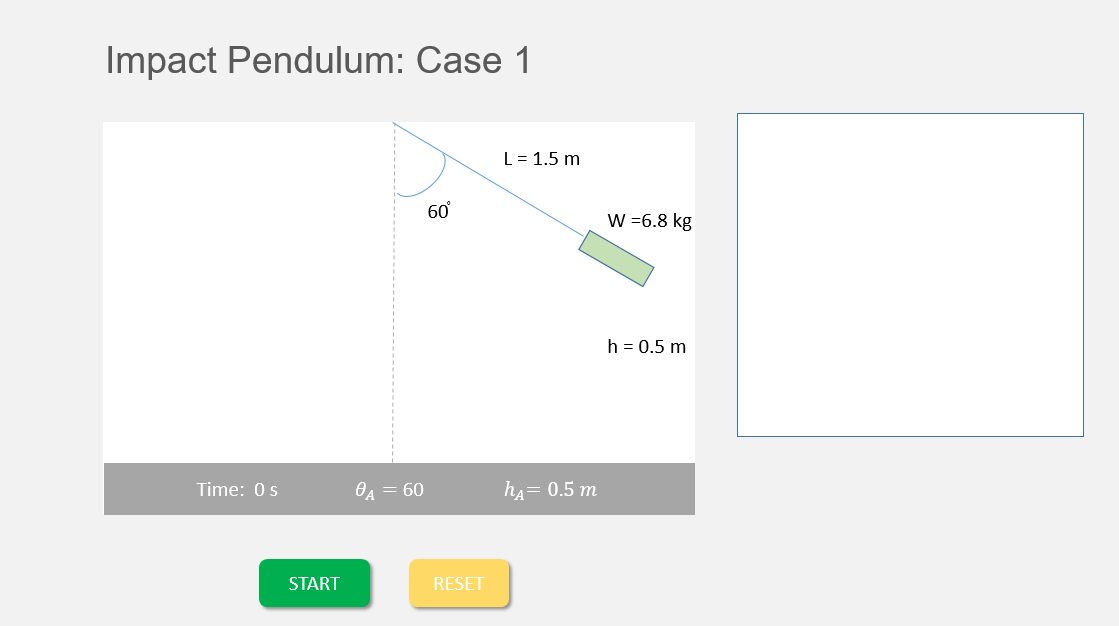
\includegraphics[width=5.5 in]{pendulum_case_1_1.png}
  \caption{Pendulum Case 1 - Before animation UI}
  \label{fig:case1_start}
\end{figure}
 
\begin{figure}[H]
  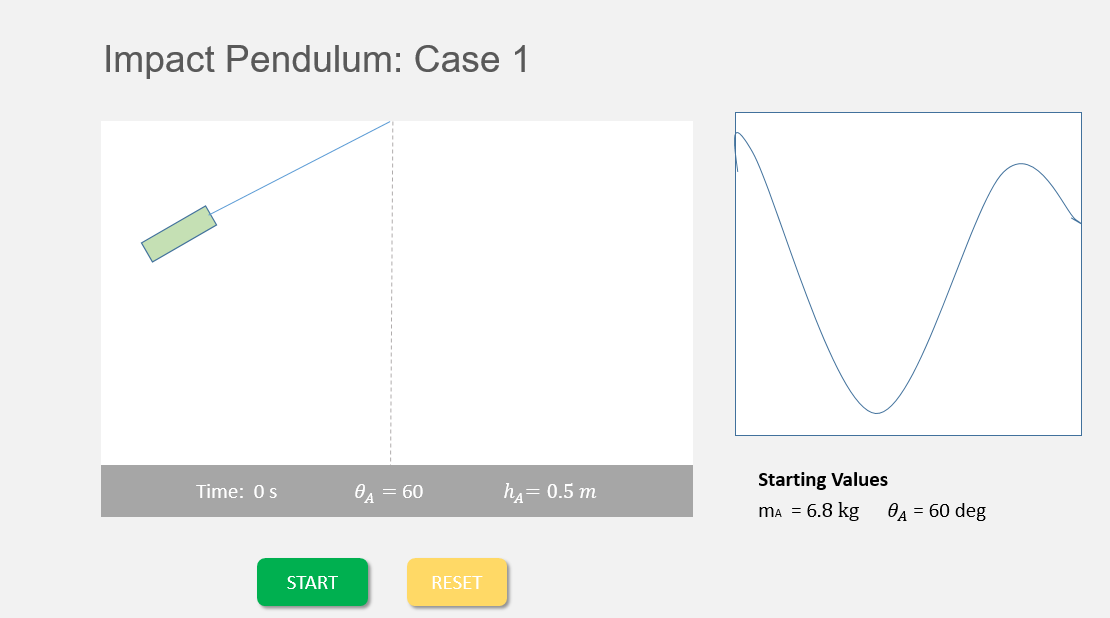
\includegraphics[width=5.5 in]{pendulum_case_1_2.png}
  \caption{Pendulum Case 1 - After animation completion UI}
  \label{fig:case1_end}
\end{figure}


\subsubsection{Function Attribute: Exploratory Mode}
The mockup of the Exploratory mode where the user can modify parameters is shown in Figure \ref{fig:explore_start} and Figure \ref{fig:explore_mid}. 
The exploratory mode components are
\begin{itemize}
  \item Start/Pause Button - Starts the simulation or pauses it 
    \item Reset Button - Resets the simulation
    \item Graph of angle vs. time 
    \item Live measurement updates  - Updates the angle and height of each weight, velocity, and the time every 0.1 seconds of the simulation
    \item Option to choose between 1 weight or 2 weights
    \item Starting parameter input sliders for the angle (degrees), length (m), weight (g), and coefficient of restitution.
\end{itemize}
\begin{figure}[H]
  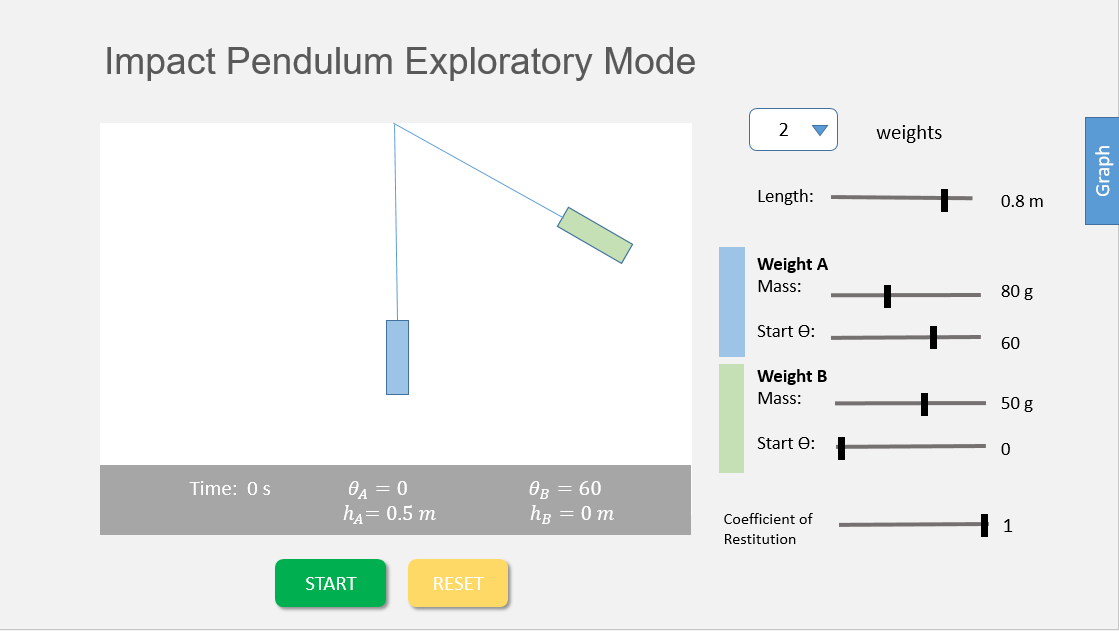
\includegraphics[width=\textwidth]{new_explore_s.png}
  \caption{Exploratory Mode Start Screen}
  \label{fig:explore_start}
\end{figure}
\begin{figure}[H]
  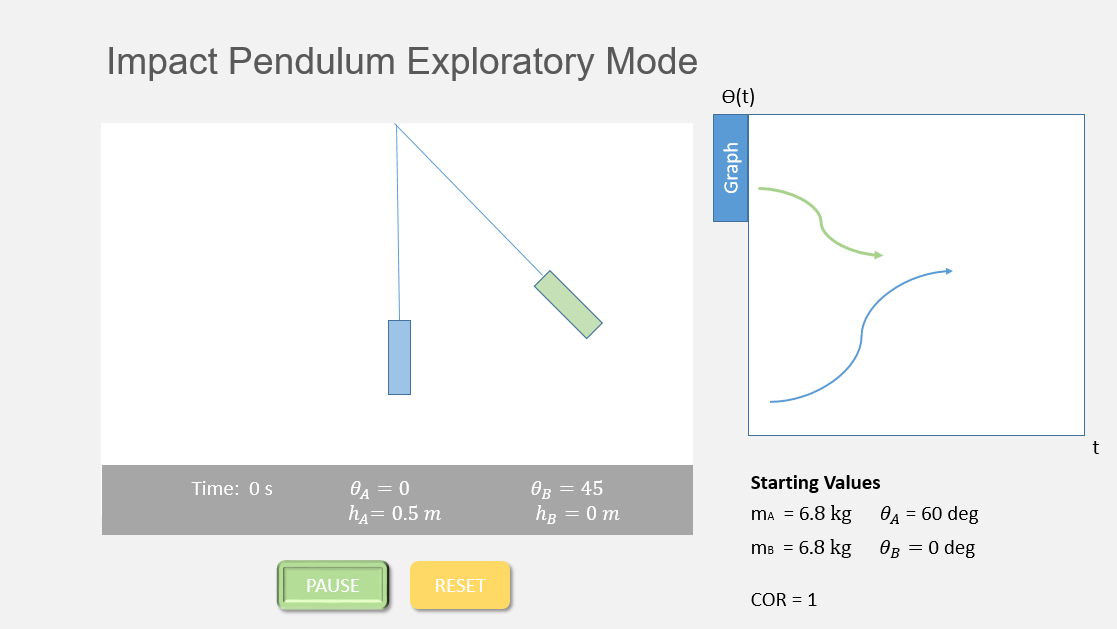
\includegraphics[width=\textwidth]{new_explore_mid.png}
  \caption{Exploratory Mode Mid Animation}
  \label{fig:explore_mid}
\end{figure}

The webpages uses HTML/CSS and Javascript to construct the start/pause/reset buttons, live measurement update tables, menu options, and the input sliders. Everything but the input sliders are constructed by HTML features: \textit{button, select, option}. 
The input sliders are constructed by the JavaScript library noUiSlider. This library provides callback functions, called whenever the users changes the slider. Whenever the user changes the slider button, the simulation world is updated to match the current values of that slider. Matter.js has features to set the object's mass and coefficient of restitution. The position of the pendulum weights are calculated based on the length of the pendulum arm and the angle. 
\begin{equation}
    x = x_p - l*sin(\theta)
\end{equation}
\begin{equation}
    y = y_p + l*cos(\theta)
\end{equation}
%collision object 
The animation receives inputs from the input sliders and the drop down menu, so user input can be limited to reasonable measurements for the pendulum system. The coefficient of restitution input will affect the pendulum game object's setting \textit{restitution} - affecting how the objects react after colliding (i.e. sticking together or not). Matter.js has a \textit{collision object} feature that has built in physical behavior and properties. 
\newline The graph of the weight's angle over time will replace the input sliders after starting the simulation. When the start button is hit, the sliders are hidden, and the graph is shown. The graph shown is based on the user's choice between angle vs time, height vs time, or velocity vs time.
The height of the weights is calculated by the equation 
\begin{equation}
    h = L - Lcos(\theta)
\end{equation}
Where L is the length of the pendulum arm, and the angle is relative to the center of the simulation.
The velocity vs time graph uses the calculated values from Matter.js. 


% End UI section **********************************

%********************************************
%  Graphing
%********************************************
\subsection{Viewpoint: Graphing}

\subsubsection{Design Concerns}
Graphs can be over stimulating if too much information is being presented to the viewer. Caution must be had when creating the graphs, so the layout is clear, and only important data points are being used.

\subsubsection{Design Elements}
 Graphs will be displayed to the screen with Chart.js, which is a lightweight JavaScript library that is free to use. Once the library is included with the script tag, a graph can be included by creating a Chart object with modifiable fields to build up your graph, such as, label for the graph's title, data for the graph's data to be graphed, and backgroundColor. After the object is made, it can be referenced to a canvas tag in order to be embedded within the web page.

\subsubsection{Function Attribute}
Graphs will be used within the UI for data visualization to provide the student with another resource to understand the interactions within the simulation.
% would a code example help here? https://www.chartjs.org/docs/latest/ 
% Any input appreciated! - Cameron

%\subsubsection{Relationship}

\subsection{Conclusion}
The core aspect of this project's development revolves around the use of the Matter.js physics library, which will be supported with the UI designs written with HTML,CSS, and JavaScripts - utilizing helper JavaScript libraries like Chart.js and noUiSlider. 
